% codigoFuenteLibroR2
% Copyright (C) 2020  J.M. Perez Zerpa, et. al.
%
% This program is free software: you can redistribute it and/or modify
% it under the terms of the GNU General Public License as published by
% the Free Software Foundation version 3 of the License.
%
% This program is distributed in the hope that it will be useful,
% but WITHOUT ANY WARRANTY; without even the implied warranty of
% MERCHANTABILITY or FITNESS FOR A PARTICULAR PURPOSE. See the
% GNU General Public License for more details.
%
% You should have received a copy of the GNU General Public License
% along with this program.  If not, see <http://www.gnu.org/licenses/>.

\chapter[Simetría y Líneas de Influencia en pórticos]{Simetría y Líneas de Influencia en pórticos}


En esta unidad se presentan dos conceptos o métodos específicos del análisis de pórticos planos.  Por una parte simetría y antisimetría, con su aplicación al análisis simplificado de pórticos planos. Por otra parte se presenta una introducción a la aplicación de líneas de influencia en pórticos hiperestáticos. %
%
Para la sección de simetría se utiliza un enfoque basado en las ecuaciones de equilibrio para obtener las condiciones mecánicas y cinemáticas dadas por la simetría, aplicándolas luego en pórticos de forma similar a como es realizado en \citep{CerveraRuiz2002ii}. %
%
La sección de Líneas de Influencia está basada en \citep{Celigueta2003}.




\section{Simetría en estructuras planas}

En esta sección se desarrollan los puntos más importantes para la consideración de simetría en el análisis de pórticos. %
%
Para la presentación se consideran pórticos planos cuya geometría tiene un eje de simetría axial. %
%
Los conceptos vistos pueden ser generalizados a estructuras tridimensionales.

\subsection{Viga sometida a cargas externas simétricas}

En la \autoref{fig:vigsim} se muestra un elemento de viga con sección transversal con inercia $I$ y área $A$, módulo de Young $E$ y largo $\ell$, el cual está sometido a cargas distribuidas y nodales simétricas respecto al punto medio de la viga (punto considerado como origen de la coordenada $x$). %

\begin{figure}[htb]
\centering
\def\svgwidth{0.9\textwidth}
\input{figs/UT4/vigasime.pdf_tex}
\caption{Esquema de viga sometiga a cargas simétricas.}
\label{fig:vigsim}
\end{figure}

Las cargas nodales pueden ser provocadas por agentes externos o bien deberse a reacciones asociadas a vínculos que restringen desplazamientos nodales. %
%
Si las cargas y las restricciones en desplazamiento (vínculos a tierra) son simétricos entonces las reacciones asociadas a dichos vínculos también lo serán. %

Se desea obtener cuales son las propiedades que cumplen las solicitaciones y los desplazamientos para este caso. %
%
Para esto se plantean las expresiones matemáticas de cada una de las hipótesis y ecuaciones disponibles y se procede a realizar el desarrollo.

\paragraph{Simetría de cargas externas}
%
Observando en la figura la simetría de las fuerzas nodales y recordando la convención de signos de la UT3 para solicitaciones internas, se tiene que la simetría es equivalente a las siguientes condiciones en las solicitaciones en los extremos:
%
\begin{eqnarray}
V \left(-\frac{\ell}{2}\right) = F_y \quad 
V\left( \frac{\ell}{2}\right) = -F_y \\
M\left( -\frac{\ell}{2}\right) = M_n \quad
M\left( \frac{\ell}{2} \right) = M_n.
\end{eqnarray}
%

Por otra parte, la simetría de la carga distribuida es equivalente a decir que la función de la carga $q(x):\left[-\frac{\ell}{2},\frac{\ell}{2} \right] \rightarrow \bbR$ es una función par. %
%
La definición de función par establece que:
\begin{equation}
q( x) = q(-x) \qquad \forall x \in \left[-\frac{\ell}{2},\frac{\ell}{2} \right].
\end{equation}

Estas relaciones representan condiciones de contorno para obtener relaciones particulares a partir de las ecuaciones de equilibrio.

\paragraph{Equilibrio puntual y relación con desplazamientos}
Se pasa a analizar la forma de las ecuaciones de equilibrio puntual, dadas por:
\begin{eqnarray}
\frac{dV}{d x} &=& q \\
\frac{dM}{d x} &=& V
\end{eqnarray}
donde nuevamente se recuerda que se utiliza la convención de signos 1 de la UT3. También se cuenta con las relaciones fuerza desplazamiento obtenidas en la UT3 a partir de la ecuación constitutiva y las hipótesis cinemáticas:
\begin{eqnarray}
\frac{d\theta}{d x} &=& \frac{M}{E I} \\
\frac{dv}{d x} &=& \theta
\end{eqnarray}



\paragraph{Equilibrio global}
Finalmente se establece la condición del equilibrio global para cualquier segmento de viga considerado. %
%
En particular se consideran las dos mitades de la viga por lo que se realiza un corte en $x=0$. %
%
El equilibrio de fuerzas verticales de la mitad derecha está dado por:
%
\begin{equation}\label{eqn:vmas}
  V(0) + \int_{0}^{\ell/2} q(u) du + F_y = 0
\end{equation}
%
donde $V(0)$ es el cortante en la sección del plano de simetría., %
%
Por otra parte también se tiene la ecuación del equilibrio de fuerzas de la mitad izquierda, dado por:
%
\begin{equation}\label{eqn:vmenos}
  -V(0) + \int_{-\ell/2}^0 q(u) du + F_y = 0.
\end{equation}
%

Considerando el cambio de variable $s=-u$ y usando que $q$ es par se tiene:
\begin{equation}
-V(0) - \int_{\ell/2}^0 q(s) ds + F_y = 0
\end{equation}
invirtiendo los límites de integración se obtiene
%
\begin{equation}
-V(0) + \int_{0}^{\ell/2} q(s) ds + F_y = 0
\end{equation}
Restando miembro a miembro la Ecuación~\eqref{eqn:vmas} se tiene
\begin{equation}\label{eqn:vex}
-V(0) - V(0) = 0\Rightarrow  \boxed{
	V(0) = 0}.
\end{equation}

% --------------------------


\paragraph{Desarrollo de cortante}
Se pasa a buscar cual es la forma del cortante $V(x)$ bajo las hipótesis consideradas. %
%
El cortante puede ser calculado integrando la primer ecuación puntual de equilibrio:
%
\begin{equation}
V(x) = \int_{0}^{x} q(u) \dif u + V(0).
\end{equation}
%
Es importante destacar que esta ecuación es equivalente a considerar el equilibrio de fuerzas verticales del segmento de viga $[0,x]$.


Usando el resultado de la Ecuación~\eqref{eqn:vex} se tiene:
\begin{equation}\label{eqn:v1}
V(x) = \int_{0}^{x} q(u) \dif u.
\end{equation}

Considerando el cambio de variable $s=-u$ se obtiene:
%
\begin{equation}
V(x) = \int_{0}^{-x} -q(-s) \dif s,
\end{equation}
%
donde se puede nuevamente ver que esto es equivalente a una ecuación de equilibrio del segmento $[-x,0]$. %
Usando que $q$ es par se tiene
\begin{equation}\label{eqn:v2}
V(x) = - \int_{0}^{-x} q(s) \dif s.
\end{equation}
%


A partir de las ecuaciones \eqref{eqn:v1} y \eqref{eqn:v2} se puede ver que:
%
\begin{equation}
V(x) = - \int_{0}^{-x} q(s) \dif s  = -V(-x)
\Rightarrow \boxed{
V(x) = -V(-x)}
\end{equation}
%
por lo que queda demostrado que $V$ es una función impar y el cortante es nulo en el eje de simetría.


\paragraph{Desarrollo de momento}
El momento interno en una sección cualquiera $x$ puede ser obtenido  a partir de la segunda ecuación puntual de equilibrio:
%
\begin{equation}
M(x) = \int_{0}^{x} V(u) \dif u + M(0).
\end{equation}
%
Realizando el cambio de variable $s=-u$ se obtiene
\begin{equation}
M(x) = \int_{0}^{-x} -V(-s) \dif s + M(0)
\end{equation}
%
y usando que $V$ es impar se tiene
\begin{equation}
M(x) = \int_{0}^{-x} V(s) \dif s + M(0) = M(-x)
\Rightarrow \boxed{
M(x) = M(-x)
}
\end{equation}
por lo que se demostró que $M$ es par.

\paragraph{Desarrollo de giro}
El giro puede ser calculado integrando la ecuación de momento curvatura:
%
\begin{equation}
\theta(x) = \int_{0}^{x} \frac{ M(u)}{EI} \dif u + \theta(0).
\end{equation}
%
Haciendo cambio de variable $s=-u$ y usando que el momento es par se obtiene:
\begin{equation}
\theta(x) = - \int_{0}^{-x} \frac{ M(s)}{EI} \dif s + \theta(0).
\end{equation}

Si se considera cada mitad de la viga por separado se puede ver que el giro del punto en el eje de simetría debería tener valores opuestos debido a la simetría de las cargas. %
%
Por otra parte por continuidad de la viga en dicho punto se cumple que los giros de ambos extremos deben ser iguales por lo que se concluye que dicho giro debe de ser nulo, por lo tanto $\theta(0) = 0$. 

Se tiene por lo tanto que:
%
\begin{equation}
  \theta(x) = - \int_{0}^{-x} \frac{ M(s)}{EI} \dif s =  -\theta(-x) \Rightarrow \boxed{\theta(x) = -\theta(-x)}.
\end{equation}
por lo que se demostró que el giro es impar y tiene valor nulo en el eje de simetría.

\paragraph{Desarrollo de flecha}
La flecha se obtiene integrando la ecuación diferencial que la relaciona con el giro:
%
\begin{equation}
v(x) = \int_{0}^{x} \theta(u) \dif u + v(0).
\end{equation}
%
Realizando el cambio de variable $s=-u$ se obtiene
\begin{equation}
v(x) = \int_{0}^{-x} -\theta(-s) \dif s + v(0)
\end{equation}
y usando que el giro es impar se tiene
\begin{equation}
v(x) = \int_{0}^{-x} \theta(s) \dif s + v(0) = v(-x)
\Rightarrow \boxed{
	v(x) = v(-x)
}
\end{equation}
por lo que se demostró que $v$ es par.

En resumen se probó que para las hipótesis establecidas, si la \textbf{carga} distribuida par $q(x) = q(-x)$ se cumple que: 
\begin{itemize}
	\item el \textbf{cortante} impar $V(x) = -V(-x)$,
	\item el \textbf{momento} par $M(x) = M(-x)$,
	\item el \textbf{giro} impar $\theta(x) = -\theta(-x)$,
	\item y la \textbf{flecha} par $v(x) = v(-x)$.
\end{itemize}


\subsubsection{Carga puntual o articulación en eje de simetría}

De forma análoga se pueden desarrollar las variantes de las ecuaciones para los casos en los que existe una carga puntual o una articulación en el eje de simetría de la viga.

En el caso de carga puntual existe una discontinuidad antisimétrica en el cortante de valor igual a la carga aplicada y en el caso de la articulación existen también una discontinuidad impar del valor del giro a cada lado de la articulación. %
%


\subsection{Pórticos planos simétricos con cargas simétricas}

El mismo razonamiento realizado para vigas puede ser extendido a pórticos, donde se debe considerar un sistema de coordenadas local $x$ continuo a lo largo de los pilares y vigas que se deseen analizar en cada etapa. %
%
El estudiante interesado en comprender en mayor profundidad el enfoque utilizado puede consultar \citep{CerveraRuiz2002ii}. %

En caso de existir una barra en el eje de simetría se obtiene un resultado equivalente al obtenido considerando una barra con la mitad de rigidez a directa, es decir con una sección transversal con la \textit{mitad de área}. %
%



En la \autoref{fig:simplifporsim} se muestra a la izquierda un pórtico simétrico con cargas simétricas aplicadas y a la derecha un pórtico equivalente obtenido a partir de las consideraciones de simetría y los resultados obtenidos. %
%
\begin{figure}[htb]
\centering
\def\svgwidth{0.8\textwidth}
\input{figs/UT4/simeport.pdf_tex}
\caption{Esquema de simplificación por consideraciones de simetría de pórtico.}
\label{fig:simplifporsim}
\end{figure}

Es importante destacar en este caso que el empotramiento deslizante considerado en el eje de simetría está asociado al hecho de que el giro es nulo por la simetría de las cargas y no necesariamente a la rigidez a flexión del pilar del eje de simetría.


\subsection{Viga simétrica con cargas externas antisimétricas}

En esta sección se presentan de forma sintética las condiciones correspondientes a estructuras \textbf{simétricas} con cargas antisimétricas (es decir impares). %

De forma análoga al caso de la viga con cargas simétricas, si las cargas son antisimétricas se cumple que:
%
\begin{itemize}
\item \textbf{carga} distribuida impar $q(x) = -q(-x)$
\item \textbf{cortante} par $V(x) = V(-x)$
\item \textbf{momento} impar $M(x) = -M(-x)$
\item \textbf{giro} par $\theta(x) = \theta(-x)$
\item \textbf{flecha} impar $v(x) = -v(-x)$
\end{itemize}

Se puede mostrar que el momento es nulo en el eje de simetría.

\subsection{Pórticos planos simétricos con cargas antisimétricas}

%Se puede mostrar que en el caso de pórticos simétricos sometidos a cargas antisimétricas se aplican consideraciones similares a las anteriores. %
%
En la \autoref{fig:simpanti} se muestra a la izquierda un pórtico con cargas antisimétricas y a la derecha un pórtico obtenido a partir de las simplificaciones de antisimetría consideradas.
%
\begin{figure}[htb]
	\centering
	\setlength{\unitlength}{0.8\textwidth}
\def\svgwidth{0.8\textwidth}
\input{figs/UT4/antisimeport.pdf_tex}
	\caption{Esquema de simplificación por consideraciones de antisimetría de pórtico.}
	\label{fig:simpanti}
\end{figure}

Es importante destacar en este caso que el apoyo deslizante considerado en el eje de simetría está asociado al hecho de que la flecha es nula por la antisimetría de las cargas y no necesariamente a la rigidez a directa del pilar del eje de simetría.

\subsection{Descomposición simetría/antisimetría}

En práctico se mostrará que, para una estructura simétrica, es posible descomponer cualquier estado de carga en suma de uno simétrico y otro antisimétrico, permitiendo simplificar el análisis de cualquier estructura simétrica.


\section{Líneas de influencia}

En esta sección se presenta un método para la determinación de líneas de influencia de reacciones y solicitaciones en estructuras hiperestáticas. %
%
El enfoque utilizado se basa en la aplicación de superposición y el Teorema de Betti (enunciado en la Sección~\ref{sec:Betti}).
%
El texto de referencia utilizado es \citep{Celigueta2003}.


Se asume que los conceptos de línea de influencia son conocidos y que se conocen los métodos utilizados para determinar las líneas de influencia en reticulados y vigas isostáticas. %
%
En caso de no contar con estos conceptos, se sugiere consultar el capítulo 10 del texto referenciado previo a leer esta sección.


Para presentar los métodos para determinación de las distintas solicitaciones se utilizará un ejemplo mostrado en la Figura~\ref{fig:ejemLI}. %
%
El esquema básico considerado consiste en un pórtico formado por elementos de pórtico de rigidez a flexión uniforme $EI$ con cuatro nodos como se muestra en la figura.

\begin{figure}[htb]
	\centering
	\def\svgwidth{0.65\textwidth}
  \input{figs/UT4/UT4_ejemploLInf_planteo.pdf_tex}
  \caption{Esquema básico de cálculo de ejemplo de líneas de influencia.}
	\label{fig:ejemLI}
\end{figure}

La flecha con un círculo representa la carga aplicada considerada móvil, en todo el tramo horizontal de la estructura y de módulo unitario.

\subsection{Líneas de influencia de reacciones}

Si se desea calcular por ejemplo la reacción vertical del nodo 3, se debe liberar el grado de libertad cinemático correspondiente. %
%
Esto es, modificar el apoyo fijo del nodo 3 por un apoyo deslizante vertical, como se muestra en la Figura~\ref{fig:ejemLIRv3}.
%

\begin{figure}[htb]
	\centering
	\def\svgwidth{0.9\textwidth}
	\input{./figs/UT4/UT4EjemploLInfRy3.pdf_tex}
	\caption{Esquemas de estados para determinación de línea de influencia de reacción.}
	\label{fig:ejemLIRv3}
\end{figure}

Los desplazamientos de cada estado son representado como $\Delta^I_{y,3}$ y $\Delta^{II}_{y,3}$ y el desplazamiento de la estructura real es calculado como
\begin{equation}
  \Delta_{y,3} = \Delta_{y,3}^I + R_{y,3} \Delta_{y,3}^{II}.
\end{equation}

La condición de apoyo fijo en 3 es $\Delta_{y,3}=0$, por lo que imponiendo esto, se puede obtener el valor de la reacción deseada:
%
\begin{equation}\label{eqn:Ry3}
  R_{y,3} = - \frac{\Delta_{y,3}^I}{ \Delta_{y,3}^{II}}.
\end{equation}

Para poder obtener un método simple de cálculo, se debe poder calcular el desplazamiento del estado I de otra forma. Para esto, se utiliza el Teorema de Betti, el cual permite establecer una relación entre el trabajo de las cargas del estado I con los desplazamientos del estado II y las cargas del estado II y los desplazamientos del estado I.

La relación establecida por el Teorema de Betti es:
%
\begin{equation}
1 \Delta_{y,P}^{II} = 1 \Delta_{y,3}^{I},
\end{equation}
donde $P$ es el punto variable de aplicación de la carga. %
%
Sustituyendo en la Ecuación~\eqref{eqn:Ry3} se tiene:
%
\begin{equation}
\boxed{
R_{y,3} = - \frac{\Delta_{y,P}^{II}}{ \Delta_{y,3}^{II}},
}
\end{equation}
%
expresión que permite calcular la línea de influencia realizando el análisis de un único EBC con un único estado de cargas estáticas.
%
En los materiales complementarios audiovisuales se mostrarán los diagramas utilizando herramientas computacionales y los desarrollos analíticos correspondientes.


\subsection{Líneas de influencia de cortantes}

Para calcular líneas de influencia de cortantes se debe liberar el vínculo cinemático correspondiente, es decir la continuidad de desplazamiento transversal.

Se considera que se desea calcular la línea de influencia del cortante (solicitación interna), en el punto medio del tramo $\circled{1}-\circled{2}$, llamado M. Para esto se libera la continuidad y se consideran los estados o esquemas básicos de cálculo mostrado en la Figura~\ref{fig:ejemLIVM}. 

\begin{figure}[htb]
	\centering
	\def\svgwidth{0.9\textwidth}
	\input{figs/UT4/EjemploLInfVM.pdf_tex}
	\caption{Esquemas de estados para determinación de línea de influencia de cortantes.}
	\label{fig:ejemLIVM}
\end{figure}

$\Delta_{y,Mi}$ y $\Delta_{y,Md}$ representan los desplazamientos transversales a la izquierda y derecha del empotramiento deslizante considerado. %
%
La condición de continuidad del desplazamiento transversal está dada por:
%
\begin{equation}\label{eqn:contDelta}
\Delta_{y,Mi} = -\Delta_{y,Md}
\end{equation}

Por otra parte, utilizando superposición, los desplazamientos en la estructura \textit{real} (con el valor de cortante $V_M$ a determinar), pueden ser escritos como:
%
\begin{eqnarray}
\Delta_{y,Mi} &=& \Delta_{y,Mi}^I + V_M \Delta_{y,Mi}^{II} \\
\Delta_{y,Md} &=& \Delta_{y,Md}^I + V_M \Delta_{y,Md}^{II} 
\end{eqnarray}

Sustituyendo en la condición de continuidad de la Ecuación~\eqref{eqn:contDelta}, se tiene:
%
\begin{equation}
\Delta_{y,Mi}^I + V_M \Delta_{y,Mi}^{II} = - \left( \Delta_{y,Md}^I + V_M \Delta_{y,Md}^{II}  \right)
\end{equation}

Por lo tanto, el cortante que garantiza la continuidad está dado por:
%
\begin{equation}
V_M  =  - \frac{ \Delta_{y,Mi}^I + \Delta_{y,Md}^{I} } { \Delta_{y,Mi}^{II} + \Delta_{y,Md}^{II} } 
\end{equation}


Usando el Teorema de Betti se tiene:
\begin{equation}
1 \cdot \Delta_{y,Mi}^I + 1\cdot  \Delta_{y,Md}^{I} = 1\cdot  \Delta_{y,P}^{II} 
\end{equation}

por lo tanto el cortante puede ser calculado como:
%
\begin{equation}
\boxed{
V_M  =  - \frac{ \Delta_{y,P}^{II}  } { \Delta_{y,Mi}^{II} + \Delta_{y,Md}^{II} } 
}
\end{equation}

En los videos complementarios se presentarán ejemplos del cálculo de líneas de influencia de cortantes.

\subsection{Líneas de influencia de momentos}

En el material complementario audiovisual se presentará el procedimiento de aplicación de \textit{Betti} para el cálculo de líneas de influencia de momentos flectores, así como también ejemplos.


\section{Ejercicios}
\setcounter{ejercicio}{0}

En todos los ejercicios presentados a continuación se deberá trabajar con estructuras simplificadas a través del uso de la simetría o antisimetría cuando corresponda, así como también, resortes equivalentes para algunas componentes estructurales. %
%



\ejercicio 

En la estructura de acero ($E=210$ GPa) de la figura, la viga continua AE está conformada por 2 PNC 18 soldados ([]) y cada uno de los tensores BF y DG tiene una sección transversal constituida por 2 barras $\phi$16. 

\begin{center}
	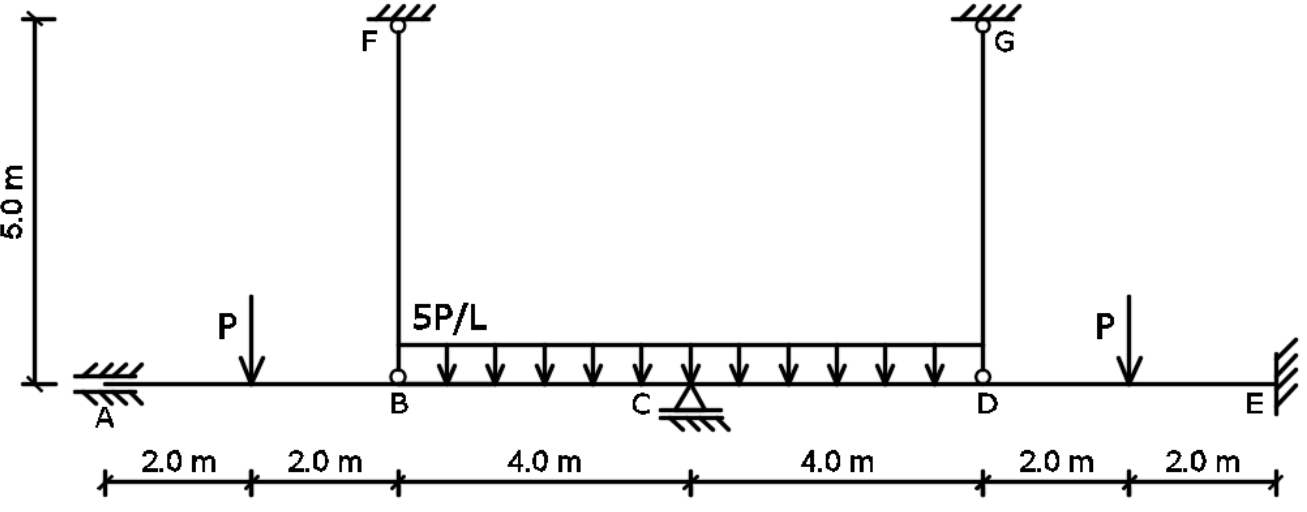
\includegraphics[width=\linewidth]{UT4ej1}
\end{center}

\parte Definir la estructura análoga más simplificada para la resolución analítica.
\parte Obtener el diagrama de solicitaciones. Considerar $P=15$ kN y $L= 4$ m.
\parte Bosquejar la deformada de la estructura.




\ejercicio

\begin{minipage}[b]{0.58\textwidth}
%
Para el marco (formado por cuatro nudos con uniones rígidas) de hormigón ($E=30$ GPa) mostrado en la figura, conformado por secciones de dimensiones $15 \times 30$ cm (inercia $I_0$) y $30\times 30$ cm (inercia $2 I_0$):
%
\parte Calcular las reacciones y trazar diagramas de solicitaciones.
\parte Bosquejar la deformada de la estructura.
\end{minipage}
~
\begin{minipage}{0.4\textwidth}
\begin{center}
	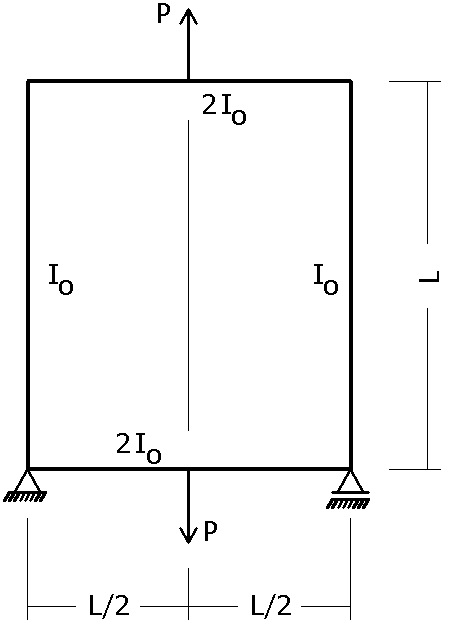
\includegraphics[width=.9\linewidth]{UT4ej2}
\end{center}
\end{minipage}




\ejercicio

Sea la estructura de la figura, conformada por barras de acero (E=210 GPa) de sección tubular de diámetro exterior $\phi =125$ mm y espesor $t=5$ mm. Considerando $P=10$ kN, se pide:



\begin{center}
	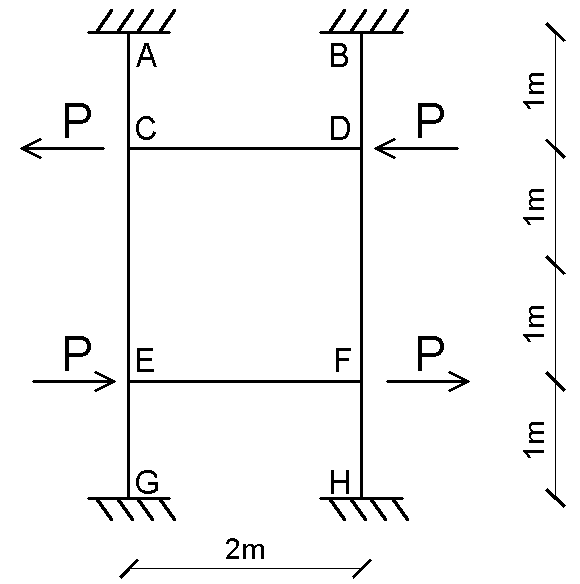
\includegraphics[width=.5\linewidth]{UT4ej3}
\end{center}

\parte Resolver la estructura y trazar diagramas de solicitaciones correspondientes.
\parte Hallar el giro de los puntos C, D, E y F. Bosquejar la deformada de la estructura.

\ejercicio

El pórtico de acero ($E=210$ GPa) mostrado en la figura está construido con perfiles con sección dada por un perfil PNI 24.

\begin{center}
	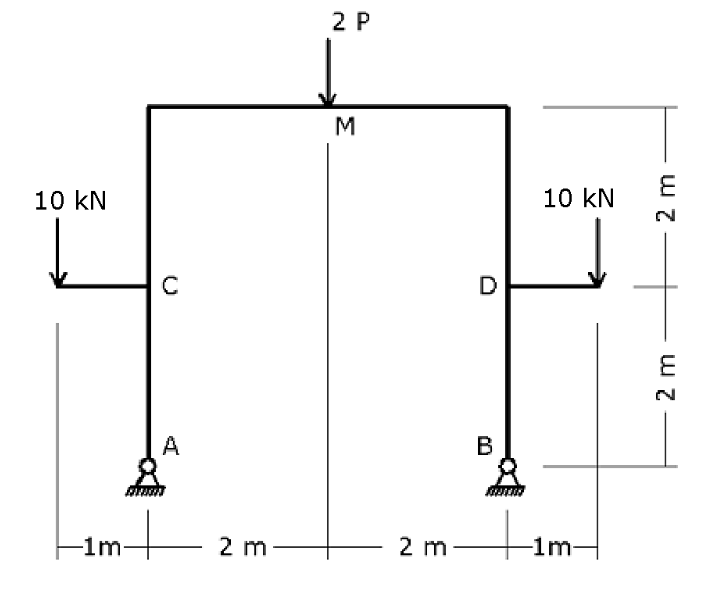
\includegraphics[width=.65\linewidth]{UT4ej4}
\end{center}

\parte Determinar el valor de $P$  para el cual las reacciones en A y B son verticales.
\parte Para ese valor de $P$, calcular el descenso de la sección M y los giros en las secciones C y  D.

\ejercicio

La estructura de acero ($E=210$ GPa) mostrada en la figura recibe la descarga distribuida de un entrepiso sobre el travesaño BC. El marco ABCD consiste en 2 perfiles PNC 20 apareados (][), mientras que el tensor AD se compone de 2 $\phi 16$.

\begin{center}
	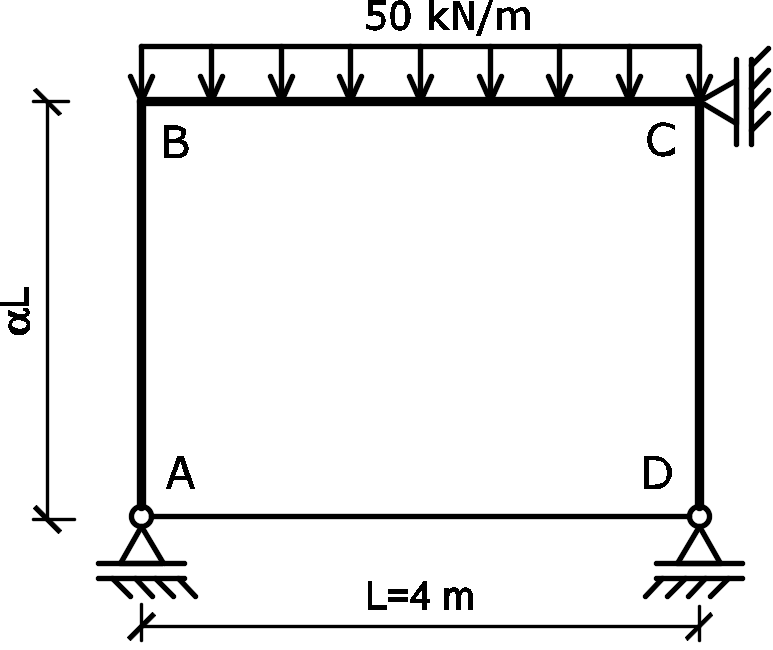
\includegraphics[width=.55\linewidth]{UT4ej5}
\end{center}

Se pide:

\parte Hallar los valores de $\alpha$ para los cuales el máximo momento que tracciona las fibras superiores y el máximo momento que tracciona fibras inferiores en el travesaño BC, son iguales en módulo. 

\parte Para el mayor valor de $\alpha$, trazar los diagramas de solicitaciones.

\ejercicio

Considere la estructura de la Figura \ref{fig61}, con $EI$ uniforme, sometida a las cargas que se indican. Se sabe que $L=2$ m y $H= 100$ kN. %
%

\begin{figure}[htb]
	\centering
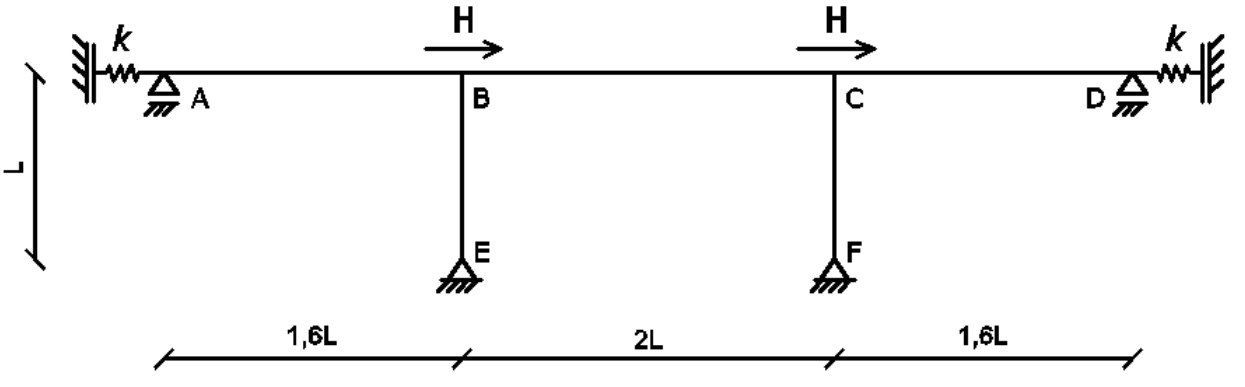
\includegraphics[width=\linewidth]{UT4ej6fig1}
\caption{Esquema de estructura.}
\label{fig61}
\end{figure}

Los pilares (barras BE y CF) están formados por tubulares de acero de diámetro exterior $\phi_{ext} = 45$ cm. %
%
La sección transversal del piso superior (barras AB, BC y CD) es una sección compuesta mostrada en la Figura \ref{fig62}. %
%
Se considera $E_{ACERO} = 210$ GPa y $E_{MADERA} = 10.5$ GPa.

\begin{figure}[htb]
	\centering
	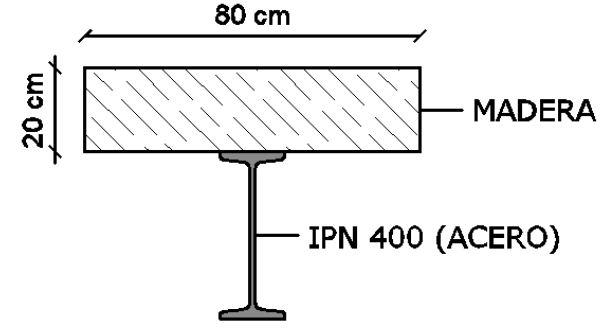
\includegraphics[width=.4\linewidth]{UT4ej6fig2}
	\caption{Esquema de sección transversal de piso superior.}
	\label{fig62}
\end{figure}
%

Se pide:

\parte Determinar el espesor $t$ de los tubulares de forma tal que se cumpla la hipótesis de EI=cte.
\parte Determinar el valor de la constante k de los resortes de forma que el desplazamiento horizontal del piso superior sea $\delta =2.6$ mm hacia la derecha.
\parte Trazar diagramas de solicitaciones y bosquejar la deformada de la estructura.



\ejercicio

La figura muestra una viga atensorada. La viga DAEBF consiste en una escuadría de madera de sección $20 \times 60$ cm, y el tensor ACB en una barra redonda de acero ($E=210$ GPa) de $\phi 16$. %
%
El puntal CE se considera infinitamente rígido. Se considera que $ E_{MADERA} = E_{ACERO} \frac{1}{30}$.

\begin{center}
	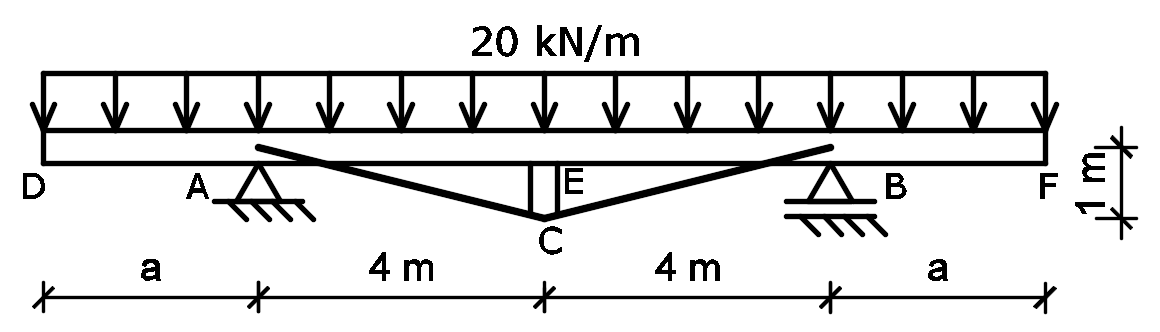
\includegraphics[width=.8\linewidth]{UT4ej7}
\end{center}

\parte Encontrar un resorte vertical en E equivalente al conjunto conformado por el tensor ACB y el puntal CE.
\parte Hallar  a tal que  los tensores estén sometidos a una tensión de $140$ MPa.
\parte Para ese valor de a, calcular la máxima tensión normal en la viga y diagramas de solicitaciones en la estructura.



\ejercicio (adicional) 

La estructura de la figura está compuesta por un marco rígido ABCD de madera ($E=10$ GPa), cuya sección es una escuadría de $15 \times 30$ cm. A su vez existe una barra bi-articulada de acero ($E=210$ GPa) que vincula la barra BC con AD en sus puntos medios, compuesta por 1$\phi$ 20.

\begin{center}
	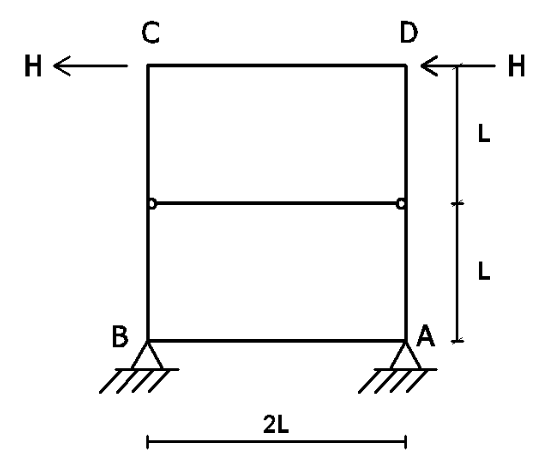
\includegraphics[width=.45\linewidth]{UT4ej8}
\end{center}

Considerando Si $H=8$ kN y $L=2$ m, se pide:

\parte Calcular el desplazamiento del punto C.
\parte Obtener los diagramas de solicitaciones de la estructura.
\parte Bosquejar la deformada de la estructura.

\ejercicio (adicional) 

La estructura de acero de la figura (E=210 GPa) está conformada por perfiles PNI 18. 

\begin{center}
	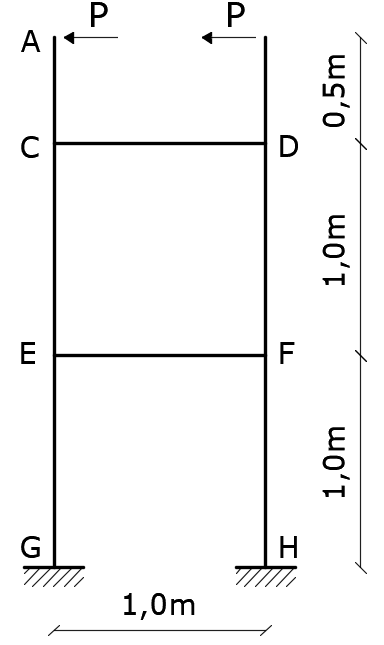
\includegraphics[width=.35\linewidth]{UT4ej9}
\end{center}

\parte Hallar reacciones y diagramas de solicitaciones si $P=15$ kN. 
\parte Bosquejar la deformada de la estructura.

\ejercicio

Sea la viga continua de la figura con $EI$=cte y con vanos de luz $l$.

\begin{center}
	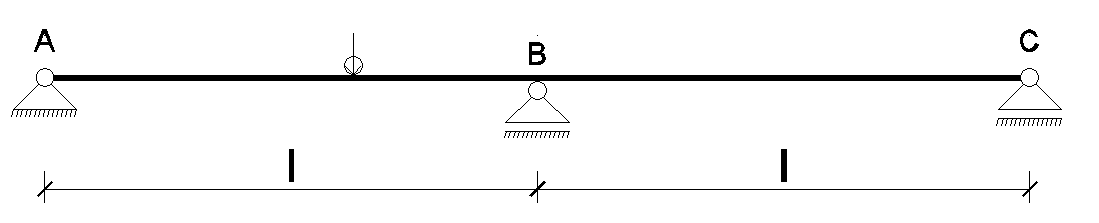
\includegraphics[width=.85\linewidth]{UT4ej10}
\end{center}

\parte Hallar la expresión analítica de la línea de influencia del momento flector $M_B$.


